\usetikzlibrary{shapes,positioning}
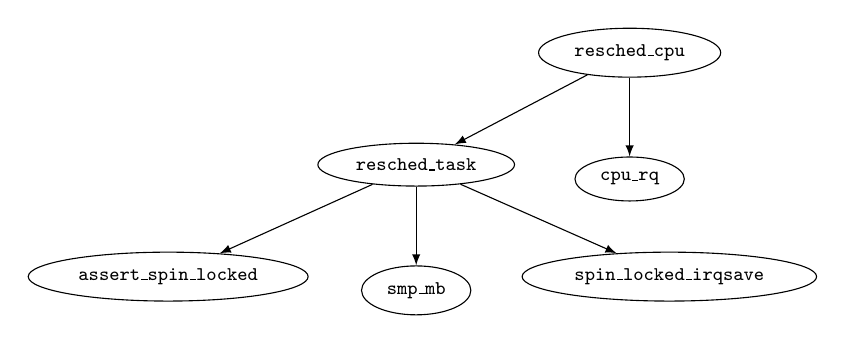
\begin{tikzpicture}[mynode/.style={ellipse,draw},myedge/.style={->,>=latex}]
  \node[mynode] (resched) {\scriptsize\tt resched\_cpu};
  \node[mynode] (rq) [below=of resched] {\scriptsize\tt cpu\_rq};
  \node[mynode] (task) [below left=of resched] {\scriptsize\tt resched\_task};
  \node[mynode] (spin) [below left=of task] {\scriptsize\tt assert\_spin\_locked};
  \node[mynode] (smpmb) [below=of task] {\scriptsize\tt smp\_mb};
  \node[mynode] (irq) [below right=of task] {\scriptsize\tt spin\_locked\_irqsave};
  \draw[myedge] (resched) -- (rq);
  \draw[myedge] (resched) -- (task);
  \draw[myedge] (task) -- (smpmb);
  \draw[myedge] (task) -- (spin);
  \draw[myedge] (task) -- (irq);
\end{tikzpicture}
